\actpart{A Royal Wedding in Dundee}% Name of Act
	{}% Background Picture
	{0cm}% X-Shift
	{0cm}% Y-Shift
	{height=\paperheight}% Graphics-Options (height, width)
	{Act01}% Short-Handle
	{test}% URL
	{test}%	Image-Name
	{test}%	Artist

\DndDropCapLine{T}{\entryfont he campaign begins in the city of Dundee, a bustling metropolis in the heart of the Kingdom of Fife. The city is in the throes of grand celebration for the wedding of Prince Angus McFife and Lady Iona McDougall. Read aloud or paraphrase:}

\begin{DndReadAloud}
	As your party crests the final hill, the sprawling city of Dundee comes into view, its towering stone walls adorned with banners of blue and gold. The air buzzes with the sounds of celebration - cheering crowds, the lively strains of music, and the toll of bells from the grand citadel in the heart of the city.
	
	The streets are alive with bustling merchants, performers, and revellers from across the kingdom, all eager to witness the union that promises to bring peace and prosperity to the land.
\end{DndReadAloud}

\section*{The Braided Unicorn}\phantomsection\addcontentsline{toc}{section}{The Braided Unicorn}
{\entryfont Nestled in the heart of Dundee, The Braided Unicorn is a sturdy stone-built inn with a weathered slate roof and timber beams, exuding a timeless charm. Above the heavy oak door hangs a beautifully carved wooden sign of a proud unicorn, its mane braided with intricate patterns, as though prepared for some ancient, regal ceremony.

Inside, the air is filled with the scent of roasted meat, strong ale, and a hint of peat smoke. A massive hearth dominates the room, its fire crackling merrily. Above the fireplace hangs an ancient great axe, rumored to have belonged to the current owner's great-grandfather.

The tavern is run by Borin Stouthammer, a stout, no-nonsense mountain dwarf with a braided iron-grey beard and a voice like rolling thunder. He keeps a keen eye on patrons from behind the polished oak bar, where rows of wooden tankards and whisky casks line the walls. Borin is quick to laugh but quicker to enforce his rules.

At the entrance, a small board proudly displays "The Braided Unicorn's House Rules":
\begin{itemize}
	\item "Nae brawling near the bar"
	\item "If ye break it, ye buy it"
	\item "Sing in tune - or buy a round for the house"
\end{itemize}

Up a creaky staircase, cozy guest rooms await with clean beds, thick quilts, and sturdy locks on the doors - perfect for a night's rest during the city's celebrations.}
{\entryfont \paragraph*{Rumours} As the party mingles, a successful DC 12 Perception (hearing) check reveals the low murmur of an intense, anxious conversation coming from a nearby table.

The source is a group of five villagers, mostly hunters and woodsfolk, huddled close and speaking in hurried, hushed tones. Their expressions range from bewilderment to dread, and the table has several empty mugs.
\begin{itemize}
	\item \textit{"I tell ye, they weren't natural unicorns - one of 'em just stared at me, eyes black as pitch."}
	\item \textit{"Aye, and those bodies... distorted they were, like something twisted the poor beasts before killing them."}
	\item \textit{"Tis nae normal wounds! Mauled, but not like any predator I've ever seen."}
	\item \textit{"It's a plague, I say. A rabid curse! Something's got into the beasts and it's spreadin'."}
\end{itemize}
The group initially looks wary but opens up if the party approaches with care (DC 15 Persuasion check, or simply buying them a round of drinks).
\begin{itemize}
	\item They describe unicorn sightings in the nearby Dundee woods, where normally noble and peaceful unicorns have been seen acting strangely - charging madly, baring teeth, and collapsing mid-gallop.
	\item Several distorted corpses of animals (and one local hunter) have been found either mauled to death or show terrifying piercing wounds.
	\item Some whisper of a "rabid curse" or a spreading sickness. Others suggest something terrifying is lurking in the woods, frightening even the unicorns.
\end{itemize}}

{\entryfont \paragraph*{Gambling Station} At the far side of the common room, a corner is dedicated to a large, well-worn oak table surrounded by mismatched chairs. Above it hangs a cracked wooden sign with the words \textbf{"Fortune's Folly"} scrawled in faded paint. The table is always surrounded by locals, travelers, and a rotating cast of suspiciously smug regulars.

Borin Stouthammer has no patience for cheaters but allows gambling as long as it doesn't disrupt the tavern. The games played here are deceptively simple, promising quick coin - a fool's trap, as the locals say.

Players can engage with Arlen, a half elf with nimble fingers and a sharper tongue, and Breeza, a halfling dressed in flashy silks, to try their fortune in varying games:

\subparagraph*{Dice Game}
A player makes contested Deception and Insight Checks against Breeza (Breeza's Deception vs. Player's Insight and Breeza's Insight vs. Player's Deception).  The winner of each round gets 2 points to their score. If Breeza and the player tie both rolls or both win one roll each, each player gets 1 point. The first player reaching 10 points in total wins the game.

\noindent\textbf{Breeza's Cheating.} Breeza (Deception +7, Insight +5) can use Arlen as a spy gaining a +5 to her Insight rolls. Players can realize that they are cheated with a successful DC 15 (-2 for each time Breeza used Arlen to cheat) Insight Check.

\subparagraph*{The Everyman's Fireball}
Tiny, wooden objects (HP 10, AC 9, immobile) are placed on the far side of the table. Each player takes a mouthful of alcohol and spits through a flame\linebreak
\vspace*{-2.5\fontdimen6\font}\hfill\\\begin{tabular}{p{0.2\textwidth}p{0.2325\textwidth}}
	\hspace*{-0.5em}\begin{tabular}[t]{p{0.2\textwidth}}
		\vspace*{0.3em}\begin{DndTable}[header=Alcoholic Drinks]{lc}
			\textbf{Drink}	& \textbf{Strength}	\\
			Weak Beer		& 1					\\
			Regular Beer	& 2					\\
			Wine			& 4					\\
			Strong Wine		& 6					\\
		\end{DndTable}
	\end{tabular}
	&
	\vspace*{0.8em}\begin{tabular}[t]{p{0.2325\textwidth}}
		{\noindent\entryfont placed between the player and the object. Before "attacking" the object, a player must make a DC 12 Dexterity roll to not burn themselves, taking \DndDice{1d4 - 1} fire damage on a failed save. The player\linebreak}
	\end{tabular}
\end{tabular}
\vspace*{-1.6\fontdimen6\font}\hfill\\then makes a ranged attack (DEX, -4 to hit; additional -2 to hit if player failed DEX save) against the wooden object, dealing \DndDice{1d6} fire damage, but not more than the drink's strength, on a hit. After each round the objects AC and the Dexterity DC increases due to the effect the drinks have on the contestants:
\begin{itemize}
	\item Objects AC: + (Drink Strength / 3) rounded down
	\item Dexterity DC: + (Drink Strength / 2) rounded down
\end{itemize}
The first to destroy the wooden object wins the game - the game is considered a tie if both are destroyed at the same time.

\noindent\textbf{Arlen's Cheating.} If Arlen (DEX +5) hits the object or nearly misses it (AC - 3), Breeza activates a contraption that will lit up the idol dealing an additional \DndDice{1d4} fire damage to the object. A DC 17 (- amount of additional damage dealt) Insight Check reveals this cheating mechanism.
}

\subsection*{An Ape-napping}
{\entryfont As the party makes their way to exit the Braided Unicorn tavern, the door bursts open with a loud \textbf{CRASH}, nearly unhinging from its frame - The party member nearest to the door must succeed on a DC 15 Dexterity Saving Throw or takes 1 bludgeoning damage from the swung open door and is knocked prone.}

\begin{DndReadAloud}
	The door slams open with a thunderous \textbf{BANG}, silencing the tavern as a figure of regal authority strides in. A grand knight, his armour polished to a mirror-like gleam and adorned with the coat of arms of Crail, surveys the room. His breath is laboured, but his presence is unshaken, exuding an aura of command.

	\textit{"WHERE are my men?!"} he mutters, more to himself than anyone else, his voice tinged with frustration and urgency.

	His eyes settle on you, narrowing for a moment as if weighing your worth. Then, stepping forward with purpose, his voice booms with authority, yet carries a regal, almost poetic cadence:

	\textit{"You there! Adventurers! I see the fire of duty in your eyes. Will you rise to the occasion, as proud sons and daughters of Dundee? A task most urgent calls, and your valour will be met with rewards worthy of your bravery. What say thee?"}
\end{DndReadAloud}

{\noindent\entryfont Should the party express their willingness to assist, the Grandmaster will give them the details of their noble task to recover the prized ape, Bobo.}

\begin{DndQuestHook}[width=0.5\textwidth - 4pt]{Rescue Bobo}
	\DndQuestHookBasics[
		location = {The Braided Unicorn Tavern, Dundee},
		quest-giver = {Ser Proletius, Grandmaster of the Knights of Crail},
		objective = {Retrieve Prince Angus McFife's stolen pet ape, Bobo, from a bandit camp in the north-eastern woods near Dundee.},
	]
	
	{\noindent\entryfont If the party succeeds on a Survival (DC 13) check, they find signs of the camp - broken branches, footprints, and scattered food - leading them toward their destination. If they fail, they instead encounter a \hyperref[monster:BanditScout]{\LinkFont{Bandit Scout}} accompanied by two \hyperref[monster:Mastiff]{\LinkFont{Mastiffs}}. The scout attempts to fight or flee, sending one mastiff back to the camp to warn the bandits. If the scout is killed, the party can find a map to the camp on his body.

		As the party approaches the camp, they find it surrounded by several traps. A Falling Net Trap is hidden among the foliage and if triggered, the net restrains the target, and a \hyperref[monster:Bandit]{\LinkFont{Bandit}} and a \hyperref[monster:Mastiff]{\LinkFont{Mastiff}} emerge to attack. The mastiff may be sent back to warn the camp if it survives. The camp is also rigged with Warning Bell Traps. If triggered, the loud sound alerts the entire camp.

		Inside the bandit camp, the party finds two \hyperref[monster:Bandit]{\LinkFont{Bandits}} and two \hyperref[monster:Mastiff]{\LinkFont{Mastiffs}} near a wooden cage containing Bobo, the stolen pet ape. If the camp is alerted - whether by a bandit's mastiff or a warning bell - additional reinforcements arrive after two rounds: a \hyperref[monster:BanditScout]{\LinkFont{Bandit Scout}}, a \hyperref[monster:Bandit]{\LinkFont{Bandit}} and another \hyperref[monster:Mastiff]{\LinkFont{Mastiff}} - if not killed before.

		The party has options for non-lethal approaches. They can attempt to infiltrate the camp, bribe the bandits, or use stealth to avoid combat. Alternatively, the party can attempt to free Bobo quietly or with force, though loud actions will attract attention.

		Bobo, frightened but alive, is in a sturdy cage (Sleight of Hand DC 15 to lockpick with thieves' tools), and the party can calm him with food or gentle handling (Animal Handling DC 13) to ensure a smooth rescue.
	}
	
	\DndQuestRewards{Upon successfully retrieving Bobo, the party receives the following rewards from King Dundax \RoyalRoman{XIII} and Prince Angus McFife:}
	{%
		{Heroic Inspiration}{}%
		{Coupon for the Wedding Festival}{%
			Each character is given a coupon, redeemable at the festival grounds for one of the following:
			\begin{itemize}
				\item A free round of the Tree Game or Dragon's Gold games
				\item A hearty free meal at one of the many stalls
			\end{itemize}
		}%
		{Private Lodging}{As a further token of gratitude, the party is given private lodging at The Braided Unicorn, rather than having to sleep in the communal quarters. This gesture signifies their growing status in Dundee and ensures them a more comfortable stay during the wedding festivities.}
		{Tournament Entry Voucher}{This voucher allows participation in the prestigious Wedding Tourney}%
		{LEVEL-UP}{At the end of the session}
	}%
\end{DndQuestHook}
	
{\entryfont\noindent When the adventurers deliver Bobo to the commanders' tent, King Dundax \RoyalRoman{XIII}, Prince Angus McFife, and Ser Proletius express their joy and gratitude. After awarding the promised rewards, Ser Proletius will single out a barbarian, fighter, ranger, or rogue (if available) in the group by giving them the Tournament Entry Voucher and set them up for a personal challenge.}

\begin{DndReadAloud}
	Ser Proletius lips curl into a confident grin. \textit{"I challenge you to enter the Wedding Tournament. Should you reach the Jousting final, regardless of the outcome, I shall reward you with a magic item from my personal possession. But should you fail..."} He pauses, letting the moment hang in the air. \textit{"You shall join me during the wedding ceremony to sing the anthem of Crail, a song of honour, glory, and tradition."}
\end{DndReadAloud}

{\entryfont\noindent If the player successfully reached the final of the Jousting Tournament they can choose between the \textbf{Cast-Off Armour} (the armour-type can be chosen by the player) or the \textbf{Shield of Expression}.

If they win the final, Ser Proletius also allows the players to fly over the city of Dundee with the mighty Eagles of Crail.}

\begingroup
	\DndSetThemeColor[PhbLightGreen]
	\begin{DndComment}{Cast-Off Armour}
		\textit{Armour (light, medium, or heavy), common}\\
		You can doff this armour as an action.
	\end{DndComment}
	\begin{DndComment}{Shield of Expression}
		\textit{Armour (shield), common}\\
		The front of this shield is shaped in the likeness of a face. While bearing the shield, you can use a bonus action to alter the face's expression.
	\end{DndComment}
\endgroup

\chapter*{Wedding Fair}\stepcounter{chapter}\phantomsection\addcontentsline{toc}{chapter}{Wedding Fair}
\DndDropCapLine{B}{\entryfont ustling with life, Dundee's wedding fairgrounds overflow with color and sound, drawing crowds into a joyous celebration that spills into nearby streets. Bright banners ripple in the breeze, lanterns glow warmly, and the tantalizing scents of roasted meats, honeyed shortbread, and mulled cider drift through the air. At the center stands a grand oak tree, its branches adorned with ribbons and lights, casting shade over the lively gathering. Roaming the grounds is the festival's famed dragon, a marvel of craftsmanship with snapping jaws, fluttering wings, and bursts of theatrical fire that delight festival-goers. Stalls brim with Highland treats, fine tartans, and handmade goods, while performers and musicians keep the festivities alive with juggling, dancing, and lively tunes.}

\begin{DndReadAloud}
	You find yourself immersed in the sights and sounds of the wedding fair. Music from fiddles and bagpipes fills the air, weaving with laughter and the chatter of excited festival-goers. Children race between stalls, clutching candied apples and pointing in delight at jugglers tossing flaming pins. The tantalizing aroma of roasted meats and sweet shortbread tempts you at every turn.

	Nearby, a massive oak tree draped in ribbons and lanterns serves as the heart of the fair. The crowd's attention shifts as the festival's dragon - a towering, lifelike marvel of wood and metal - stirs. Its wings ripple and its jaws snap with dramatic flair eliciting gasps and cheers from the crowd.

	As the sun dips below the horizon, lanterns and torches bathe the fairgrounds in a golden glow. Laughter and awe ripple through the throng as the magic of the festival fully takes hold, drawing you deeper into its spellbinding atmosphere.
\end{DndReadAloud}

\section*{Dragon's Gold}\phantomsection\addcontentsline{toc}{section}{Dragon's Gold}
\textbf{Entry Fee:} 1 GP\\
{\entryfont The Dragon's Gold is the crown jewel of the festival, a dazzling and immersive event that draws crowds of eager participants and onlookers to the central plaza. The centrepiece of this spectacle is the magnificent dragon itself, a towering construct of painted paper, wood, and metal. Adorned with shimmering scales in vibrant reds, greens, and golds, the dragon moves with startling realism. Clever mechanisms allow its angular head to snap and jerk, its wooden wings to flutter with a show of might, and its mouth to "breathe fire" in the form of colourful ribbons and occasional bursts of magical smoke. The creature prowls menacingly near its sprawling treasure hoard, exuding an air of majesty and danger that captivates the entire square.}

\subsection*{Mechanics}
{\entryfont The Dragon's Gold game takes place in a 50-foot radius playing area, covered in thick layers of hay to conceal scattered treasures. At the heart of the area lies the 15-foot radius Inner Hoard, where the most coveted prizes are clustered. However, this inner zone is guarded by the festival dragon, which relentlessly defends its treasures.}

\begin{DndMonster}[width=0.5\textwidth]{Festival Dragon}
	\DndMonsterType{Large Construct, neutral good}
	
	% If you want to use commas in the key values, enclose the values in braces.
	\DndMonsterBasics[
		armor-class = {16},
		hit-points  = {\DndDice{9d10 + 36}},
		speed       = {20 ft.},
	]
	
	\renewcommand{\AbilityScoreSpacer}{~}
	\DndMonsterAbilityScores[
		str = 7,
		dex = 7,
		con = 18,
		int = 8,
		wis = 18,
		cha = 20,
	]
	
	\DndMonsterDetails[
		saving-throws = {CON +8, CHA +9},
		skills = {Insight +8, Intimidation +9, Perception +8},
		%damage-vulnerabilities = {cold},
		%damage-resistances = {bludgeoning, piercing, and slashing from nonmagical attacks},
		%damage-immunities = {poison},
		senses = {Passive Perception 18},
		%condition-immunities = {poisoned},
		languages = {-},
		challenge = -,
		proficiency-bonus = +4,
	]
	
	\DndMonsterSection{Traits}
    \DndMonsterAction{Operative Mastery}
    The Festival Dragon must be operated by a group of at least 6 people. If the Festival Dragon is operated by a properly trained performing team, its AC is increased by 2 and gains a bonus of +4 to each melee attack and damage roll.
    
	\DndMonsterAction{Non-Lethal Attacks}
	Each attack the Festival Dragon makes is considered non-lethal
	
	\DndMonsterAction{Friendly Nature}
    The Festival Dragon is usually friendly towards children and only chases them away, unless they get too greedy.
	
	\DndMonsterSection{Actions}
	\DndMonsterAction{Multiattack}
	The Festival Dragon makes one Claw Attack and one Bite or Tail Attack.
	
	\DndMonsterAttack[
		name=Claw,
		distance=melee, % valid options are in the set {both,melee,ranged},
		%type=weapon, %valid options are in the set {weapon,spell}
		mod=-2,
		reach=5,
		%range=20/60,
		targets=one target,
		dmg=\DndDice{1d4 - 2},
		dmg-type=slashing,
		%plus-dmg=\DndDice{1d6},
		%plus-dmg-type=poison,
		%or-dmg=,
		%or-dmg-when=,
		extra={ (minimum of 1 damage)},
	]
	
	\DndMonsterAttack[
		name=Bite,
		distance=melee, % valid options are in the set {both,melee,ranged},
		%type=weapon, %valid options are in the set {weapon,spell}
		mod=-2,
		reach=5,
		%range=20/60,
		targets=one target,
		dmg=\DndDice{1d6 - 2},
		dmg-type=piercing,
		%plus-dmg=\DndDice{1d6},
		%plus-dmg-type=poison,
		%or-dmg=,
		%or-dmg-when=,
		extra={ (minimum of 1 damage)},
	]
	
	\DndMonsterAttack[
		name=Tail,
		distance=melee, % valid options are in the set {both,melee,ranged},
		%type=weapon, %valid options are in the set {weapon,spell}
		mod=-2,
		reach=20,
		%range=20/60,
		targets=one target,
		dmg=\DndDice{1d6 - 2},
		dmg-type=bludgeoning,
		%plus-dmg=\DndDice{1d6},
		%plus-dmg-type=poison,
		%or-dmg=,
		%or-dmg-when=,
		extra={ (minimum of 1 damage)},
	]
	
	\DndMonsterAction{Breath Weapon (Recharge 5 Rounds)}
	Each creature in a 30ft. long, 5 ft. wide line must make a DC16 Dexterity Saving Throw or are instantly out of the Dragon's Gold game.
	
	\DndMonsterSection{Reactions}
	\DndMonsterAction{Automated Construct}
	The Festival Dragon can make one attack of opportunity with each of its front limbs, mouth, and tail.
\end{DndMonster}

{\entryfont\noindent Participants enter the game unarmed and unarmoured, with no equipment allowed. The use of magic is strictly prohibited, and contestants may not harm or attack one another under any circumstances, preserving the festive nature of the game.

Each round lasts 2 minutes (20 rounds in total). Contestants have this time to search for and claim as much treasure as they can manage.

To locate treasures, contestants may perform one of the following actions:
\begin{itemize}
	\renewcommand\labelitemi{\textbf{\textbullet}}
	\item \textbf{Spot Check (Perception):} Roll against a DC20 Check to locate a treasure anywhere in the play area (DC15 if searching within the Inner Hoard).
	\item \textbf{Search Check (Perception):} Roll against a DC10 Check to locate a treasure in a specific 5-foot square. Searching in this way within the dragon's reach provokes an Attack of Opportunity from the dragon.
\end{itemize}
If a contestant succeeds on either check, they can roll on the Treasure Table to determine the item found.

Contestants may continue to search and gather treasure for as long as they wish, carrying as many items as they can manage. However, treasures are forfeited if a contestant is struck by the dragon's attack and "killed". To remain in the spirit of the game, "dead" contestants are expected to leave the game when they are struck and may not interact with the hoard further, though they can remain in place as casualties for the remainder of the game.}

{\entryfont\noindent Contestants may leave the treasure hoard at any time, taking their gathered loot with them. Once a contestant leaves the playing area, they cannot re-enter. Leaving the area ends their participation in the game.\\\\
The balance of greed and caution defines the game: contestants must weigh the temptation of more treasures against the risk of provoking the dragon's wrath. The most daring and resourceful participants will walk away with riches, but those who overreach may lose everything!}

\begin{DndTable}[header=Treasure Table]{lXX}
\textbf{d100}	& \textbf{Outer Hoard (value)}							& \textbf{Inner Hoard (value)}	\\
01-10			& A small mound of 3d6 cp								& A mound of 5d6 sp				\\
11-20			& A shell bracelet (2 sp)								& Costume jewellery (1 gp)		\\
21-30			& A bag filled with coloured stones and marbles (5sp)	& A finely article of clothing, tied with ribbon (5 gp) \\
31-40			& A wreath of flowers and ribbons (2 sp)				& A large box that holds many rich candies (2gp) \\
41-50			& An embroidered cloth with a picture (1 gp)			& Bronze jewellery set with semi-precious stones (5gp) \\
51-60			& A wooden token good for a free meal at a local restaurant (5sp)	& A dagger or short-sword in sheath (10 gp) \\
61-70			& A toy sword painted silver (2 sp)						& A metal flask filled with spirits (2 gp) \\
71-80			& A gold coin (1 gp)									& A pretty doll or toy (5 gp) \\
81-90			& Some type of art supply, like inks, pens, fancy wood, or paint (3 gp)	& A common item made of silver or gold, like a needle (10 gp) \\
91-100			& Roll on the Inner Hoard table at +10					& Fancy jewellery or clothing (50 gp)
\end{DndTable}

\begin{DndOptionalRule}{Attack the Dragon}
	The Festival Dragon can be attacked during the Dragon's Gold Game with weapons and weapon-like items that are found during the game. However, it is not allowed to use any kind of magic to damage the construct.
\end{DndOptionalRule}

\section*{Tree Game}\phantomsection\addcontentsline{toc}{section}{Tree Game}
\textbf{Entry Fee:} 1 GP\\
{\entryfont The Tree Game is a lively and challenging test of accuracy and skill, where contestants attempt to claim prizes nestled among the high branches of a towering tree. Using arrows, handaxes, or throwing knives, competitors aim for trinkets, baubles, and even valuable treasures carefully lodged within the tree's limbs. Each well-placed strike sends a prize tumbling gracefully to the ground, greeted by the crowd's cheers - or the envious gazes of onlookers hoping for their turn.}

\begin{DndReadAloud}
	Before you stands a majestic oak, its sprawling branches adorned with glittering prizes that catch the light like stars in the daylight. Trinkets dangle from ribbons and strings, while more valuable treasures are wedged tightly into crooks and knots high above. The lower branches sway gently with small, easy-to-reach prizes, while the loftiest rewards glint enticingly just out of easy range. Contestants gather at the base of the tree, readying their arrows, handaxes, or knives as the crowd murmurs in anticipation.

	\textit{"Step forward and take your shot!"} calls the event's master of ceremonies. \textit{"What will you claim from the tree's bounty - luck, skill, or sheer determination?"}

	The air hums with excitement as the first competitor lines up their throw, aiming to send fortune falling from the great tree's branches.
\end{DndReadAloud}

\subsection*{Mechanics}
{\entryfont In the Tree Game, contestants are tasked with dislodging prizes tied to the branches of the grand festival tree using borrowed weapons provided by the game organizers. Each participant may choose either a shortbow with 5 arrows or two handaxes, both of which must be returned at the end of the game. Over the course of five rounds, contestants attempt to target and knock down the dangling prizes, each taking a single shot or throw per round.

Using the shortbow requires precise aim, as contestants must hit the harder AC (standard-AC +2) listed in the Prize Table to sever the ribbons holding the prizes in place. Conversely, handaxes rely on brute force, allowing contestants to attack against the standard AC of the target. Regardless of the weapon used, any prize that is successfully dislodged and falls to the ground is immediately claimed by the contestant.}

\begin{DndTable}[header=Prize Table]{llX}
\textbf{Height}	& \textbf{Effective AC}			& \textbf{Prize}												\\
10-24 ft		& 11 (13)						& Dart, Bucket, Piton, Signal Whistle							\\
25-39 ft		& 13 (15)						& Ladder, Sling Bullets (40), Sling								\\
40-44 ft		& 15 (17)						& Javelin, Lamp, Blanket, Sealing wax							\\
45-49 ft		& 18 (20)						& Arrows (20), Crossbow Bolts (20), Hammer, Caltrops (bag of 20)\\
50 ft +			& 18 (20)						& Padded Armour, Handaxe, Pike, Healer's kit					\\
\end{DndTable}

\begin{DndOptionalRule}{Losing Thrown Item}
	Critical Failure (NAT 1) leads to the thrown item to be stuck in the tree as well, and needs to be retrieved/dislodged in a similar manner like the prizes. Otherwise it will be lost to the game.
	
	For each borrowed hand axe lost during the game the contestant has to pay 10GP (40GP for a lost shortbow).
\end{DndOptionalRule}
\chapter*{Wedding Tourney}\stepcounter{chapter}\phantomsection\addcontentsline{toc}{chapter}{Wedding Tourney}
\DndDropCapLine{T}{\entryfont he Wedding Tourney celebrating the union of Angus McFife I and Iona McDougall has brought an air of excitement and festivity to Dundee. The grand event unfolds with a series of thrilling competitions, drawing skilled participants and eager spectators from across the land. The day's revelry begins with an archery contest and progresses through feats of strength and skill, including the long throw and the challenging log chop. Competitors earn points in each event based on their finishing positions, with their accumulated scores determining the seeding for the climactic jousting competition. In this final contest of valour and chivalry, the ultimate winner of the tourney will be crowned, marking the joyous celebration's triumphant conclusion. The point-scoring\linebreak}

\vspace*{-4.6\fontdimen6\font}\hfill\\\begin{multicols}{2}
{\entryfont \noindent system for the Wedding Tourney is designed to reward consistent performance across the Archery, Long Throw, and Log Chopping competitions. Competitors earn points based on their\linebreak}
\vspace*{-2.2em}\begin{DndTable}[header=Point Scoring System]{lXr}
\textbf{Rank}	&& \textbf{Points}	\\
1st				&& 10				\\
2nd				&& 8				\\
3rd				&& 6				\\
4th				&& 4				\\
5th				&& 2				\\
6th				&& 1				\\
\end{DndTable}\\
\end{multicols}
\vspace*{-4.3\fontdimen6\font}\hfill\\

{\noindent\entryfont finishing positions in each event, with the highest total scores determining their seeding for the jousting competition.}

\section*{Bullseye's Glory}\phantomsection\addcontentsline{toc}{section}{Bullseye's Glory}
{\entryfont The archery competition marks the opening event of the Wedding Tourney, testing the precision and steady hands of each competitor. Standing 80 feet away from a stationary target, each archer must demonstrate their mastery over the shortbow, aiming true to score as many points as possible. Crowds gather to watch as the competitors take their shots one by one, the rhythmic twang of bowstrings ringing through the air as arrows fly toward the bullseye. This contest of skill requires calm focus and careful aim, setting the tone for the challenging events to follow.}

\subsection*{Mechanics}
{\entryfont In the archery competition, each contestant has four shots to score points based on their aim and accuracy. To make each shot, competitors roll an attack against the target, with their point total determined by the roll's outcome, as detailed in the provided Scoring Table. All competitors must use an unenchanted shortbow, provided by the tourney organizers, to ensure fair play; any archer found using enchanted equipment will be immediately disqualified.}
\begin{DndTable}[header=Archery Scoring]{lXX}
\textbf{Attack Roll}	& \textbf{Location}		& \textbf{Points}	\\
less than 8				& Miss					& 0					\\
8+						& Outer Ring			& 1					\\
11+						& Middle Ring			& 3					\\
14+						& Inner Ring			& 5					\\
17+						& Bullseye				& 10				\\
NAT20					& Split another Arrow	& 10 + \textit{Crowd Roar*}	\\
\end{DndTable}
{\footnotesize * \textit{Crowd Roar} gives a +2 to the next attack roll in this competition.}
\vfill\eject
\begin{tikzpicture}[remember picture, overlay]%
	\node[xshift=0.25cm, yshift=0.25cm, anchor=north east] at (current page.north east) {\includegraphics[width=.6\paperwidth]{%
		images/Landscape/Archery_Competition%
	}};%
\end{tikzpicture}%
\hfill\\ \\ \\
\begin{DndTable}[header=Archery Ranking]{lXl}
\textbf{Rank}	& \textbf{Name}					& \textbf{Points}	\\
1st				& Ewan MacRae of Dunkeld		& 28				\\
2nd				& Gavin Buchanan				& 19				\\
3rd				& Rory MacTavish				& 14				\\
4th				& Alasdair MacLeod				& 8					\\
5th				& Hamish "Halfwit" McGregor		& 1					\\
\end{DndTable}

\section*{Hurl of Might}\phantomsection\addcontentsline{toc}{section}{Hurl of Might}
{\entryfont The Long Throw Competition is a test of raw power, technique, and endurance, as competitors attempt to throw a series of progressively heavier and more unwieldy objects as far as possible. Each object presents a unique challenge, requiring not only physical strength but also skillful control to reach impressive distances. Spectators gather eagerly along the marked field, cheering as each competitor heaves their object through the air, striving for the farthest distance in each throw. This contest celebrates feats of might and mastery, with each participant vying to surpass their rivals in sheer throwing range.}

\subsection*{Mechanics}
{\entryfont In the Long Throw Competition, contestants must throw four distinct objects, each with its own weight and difficulty, as outlined in the provided table. Each competitor has two attempts with each object, and only the best throw for each object counts toward their total score. Each throw requires a DC 10 check to clear the first range increment, and every additional 4 points above the DC increases the throw's range by one increment, as defined in the table. The contestant can use specific skills (also noted in the table) to attempt each throw. If the object's weight exceeds twice the contestant's Strength Score in pounds, they must roll with disadvantage due to the strain of hefting the object. The contestant's gain points for each distance increment, with the competitor achieving the greatest total declared the victor of the Long Throw Competition.}

\begin{DndTable}[header=Thrown Objects]{lllX}
\textbf{Object}	& \textbf{Range}				& \textbf{Weight}		& \textbf{Skill(s)}					\\
Javelin			& 30 ft.						& 2 lbs					& STR								\\
Discus			& 20 ft.						& 5 lbs					& Athletics (STR), Acrobatics (DEX)	\\
Stone			& 10 ft.						& 18 lbs				& STR, DEX							\\
Halfling		& 5 ft.							& 30 lbs				& STR								\\
\end{DndTable}

\begin{DndTable}[header=Long Throw Ranking]{lXl}
\textbf{Rank}	& \textbf{Name}					& \textbf{Points}	\\
1st				& Ewan MacRae of Dunkeld		& 13				\\
2nd				& Alasdair MacLeod				& 10				\\
3rd				& Rory MacTavish				& 6					\\
4th				& Gavin Buchanan				& 4					\\
5th				& Hamish "Halfwit" McGregor		& 2					\\
\end{DndTable}

\section*{Timber Trial}\phantomsection\addcontentsline{toc}{section}{Timber Trial}
{\entryfont The Log Chopping competition is a thrilling display of strength, stamina, and quick decision-making, as contestants race against the clock to chop through as many logs as they can in a single minute. With logs standing at regular intervals, participants must strike quickly and move swiftly to cover the ground between each target, chopping one after another in a relentless rhythm. Spectators cheer on as wood chips fly and axes swing, creating an intense spectacle of determination and power. The choice of weapon might play a key role, as each contestant must decide between speed and force, adjusting their approach to maximize their tally. Only the most determined and strategic log chopper will claim victory in this demanding event.}

\subsection*{Mechanics}
{\entryfont In the Log Chopping competition, contestants have one minute (10 rounds) to destroy as many logs as possible. Each log has an AC of 15 and 18 HP, challenging competitors to balance force and accuracy with each swing. The logs are spaced 10 feet apart, requiring contestants to move to the next log after each one is destroyed. At the start of the competition, contestants select a weapon from the provided weapon rack, which holds 2 \textbf{Handaxes} (1d6 slashing, light), a \textbf{Battleaxe} (1d8 (1d10 versatile) slashing), and a \textbf{Greataxe} (1d12 slashing, heavy, two-handed). They may switch weapons during the contest, but doing so requires a full round to return to the rack and select a new weapon. The contestant who destroys the most logs within the allotted time is declared the winner, with any ties broken by the lowest HP remaining on the last partially damaged log.}

\begin{DndTable}[header=Log Chopping Ranking]{lXl}
\textbf{Rank}	& \textbf{Name}					& \textbf{Points}	\\
1st				& Hamish "Halfwit" McGregor		& 10*				\\
2nd				& Ewan MacRae of Dunkeld		& 5 (18 HP)			\\
3rd				& Alasdair MacLeod				& 3 (12 HP)			\\
4th				& Rory MacTavish				& 2	(6 HP)			\\
5th				& Gavin Buchanan				& 1 (12 HP)			\\
\end{DndTable}
{\footnotesize * Hamish has used an illegal Adamantine Axe for this challenge and will be disqualified after the competition}

\section*{The Grand Joust}\phantomsection\addcontentsline{toc}{section}{The Grand Joust}
\begin{DndReadAloud}
	Before you stretches the grand jousting arena, a testament to the kingdom's dedication to noble sportsmanship and spectacle. The tiltyard is a long, sandy stretch bordered by wooden rails, with pennants in vibrant colors fluttering from high poles. Rows of wooden stands rise on either side, packed with eager onlookers waving banners of the Kingdom of Fife. At the center of the stands, the royal box gleams with ornate carvings and golden accents, where the bride and groom sit with their court, overseeing the proceedings with regal anticipation. Squires and attendants scurry along the perimeter, preparing horses and lances while the competitors mount up for the first tilt. The air is electric with the sound of cheering, the smell of trampled earth, and the thrill of impending glory.
\end{DndReadAloud}

\subsection*{Mechanics}
{\entryfont Based on their performances in the earlier contests - the Archery, Long Throw, and Log Chop - the champions have been seeded: the first-ranked competitor will face the fourth, and the second will challenge the third. Only the victors of these matches will move on to the final joust to determine the champion of the tourney.}
\subsubsection*{Mount Familiarization}
{\entryfont Before engaging in the joust, each competitor must take time to familiarize themselves with their mount. This crucial moment allows them to build a bond of trust and control, ensuring their steed responds with precision during the high-stakes contest.}

{\entryfont Each participant must make a DC 15 Animal Handling Check to gauge how well they connect with their mount.
\begin{itemize}
	\renewcommand\labelitemi{\textbf{\textbullet}}
	\item \textbf{Success:} The rider gains a +1 bonus to their first Ride (Constitution) check during the joust.
	\item \textbf{Critical Success (Natural 20):} The rider gains a +2 bonus to their first Ride (Constitution) check and an additional +1 bonus to a potential subsequent Ride (Constitution) check.
	\item \textbf{Critical Failure (Natural 1):} The rider suffers a -2 penalty to their first Ride (Constitution) check and a -1 penalty to all subsequent Ride (Constitution) checks for the duration of the competition.
\end{itemize}}
\subsubsection*{The Joust}
{\entryfont After familiarizing themselves with their mounts, the contestants ride onto the tiltyard for the main event. The jousting competition is a dramatic test of precision, strength, and endurance. Riders charge toward one another, their tourney lances poised to strike, as the crowd cheers in anticipation of every thunderous impact.

Contestants use specially crafted tourney lances provided by the organizers. These lances deal 1d4 piercing (non-lethal) damage. If a rider deals more than 10 damage in a single round, the lance shatters spectacularly, earning the rider a +2 bonus to their next attack roll as the crowd cheers their impressive display of skill and power.

The use of magic during the joust is strictly forbidden and results in immediate disqualification.

Each pass between the two contestants is resolved through simultaneous strikes. Riders may choose one of the following attack strategies for their turn:

\begin{itemize}
	\renewcommand\labelitemi{\textbf{\textbullet}}
	\item \textbf{Aim at Helmet:}
	\begin{itemize}
		\item Attack Roll Penalty: -8 to attack roll.
		\item If the attack lands, the opposing rider must make a Ride (Constitution) Check with a DC of 15 + damage dealt to stay mounted.
	\end{itemize}
	\item \textbf{Crouch defensively:}
	\begin{itemize}
		\item Attack Roll Penalty: -4 to attack roll.
		\item The rider gains a +4 bonus to their Ride (Constitution) Check if struck.
	\end{itemize}
\end{itemize}

\noindent When struck by an opponent's lance, a rider must make a Ride (Constitution) Check (DC 5 + damage dealt) to remain in the saddle. Any rider reduced to 0 HP will automatically fail this check.

\noindent The unseated rider must succeed on a DC 15 Athletics or Acrobatics Check to land safely. On a failed check, the rider takes 1d6 bludgeoning damage from the fall.

If both riders remain mounted after a pass, the joust continues into another round. The DC for all subsequent Ride (Constitution) Checks increases by +2 after each round to represent the mounting tension and fatigue of the contest. The joust ends when only one rider remains mounted. That rider is declared the winner.

If both riders are unseated in the same round, the contest escalates into a melee duel to determine the victor. Both contestants are armed with blunt shortswords (1d4 bludgeoning, non-lethal) provided by the organizers. The duel continues as a standard one-on-one melee fight, with both riders retaining the hit points and damage accumulated during the joust. The first contestant to submit or fall unconscious loses the joust.}

\subsection*{"Party-cipation"}
{\entryfont The jousting finale may be centred on one member of the party, but the bonds of friendship and camaraderie run deep. This optional rule allows the rest of the party to actively contribute to their champion's performance, giving them a chance to support and influence the outcome in meaningful ways. Whether through cheering, strategizing, or even small magical gestures (within the festival's rules, of course), the party's involvement can turn the tide in a close contest. Following are some ideas that can be implemented:
\begin{itemize}
	\renewcommand\labelitemi{\textbf{\textbullet}}
	\item \textbf{Hype up the Crowd}\\
	The party members can use their turn to cheer, chant, or otherwise encourage their champion. Doing so requires a successful Charisma (Performance) Check DC 13 to hype up the crowd and giving the following benefits:
	\begin{itemize}
		\renewcommand\labelitemii{\textbf{\textbullet}}
		\item \textbf{Success}\\
		The champion gets a +2 bonus on either the next attack roll or the next Ride (Constitution) Check.
		\item \textbf{Critical Success}\\
		The champion also gains temporary hit points equal to the party members' highest Charisma modifier (minimum of 1).
		\item \textbf{Critical Failure}\\
		The next attack roll and a possible Ride (Constitution) Check are made with disadvantage.
	\end{itemize}
\end{itemize}
\vfill\eject
\begin{itemize}
	\renewcommand\labelitemi{\textbf{\textbullet}}
	\item \textbf{Crowd Manipulation}\\
	A particularly charismatic party may attempt to rally the crowd to their champion's favour. This requires a Charisma (Persuasion) or Charisma (Deception) Check (DC 20).
	\begin{itemize}
		\renewcommand\labelitemii{\textbf{\textbullet}}
		\item \textbf{Success}\\
		The crowd becomes fully invested in the champion's success, granting a +2 bonus to their attack rolls for the next two rounds.
		\item \textbf{Critical Success}\\
		The crowd's overwhelming support inspires the champion, giving them advantage on all checks and attack rolls for the next two rounds.
		\item \textbf{Failure}\\
		The crowd's disapproval leads to the champion being distracted, having disadvantage on the next attack and potential Ride (Constitution) check.
		\item \textbf{Critical Failure}\\
		The crowd immensely disapproves of the champion, giving them disadvantage on all checks and attack rolls for the next two rounds.
	\end{itemize}
\end{itemize}
}
\subsubsection*{Boon of the Crowd}
{\entryfont If the party influenced the match (through cheering or crowd manipulation), the champion gains the following boon:
\begin{itemize}
	\item The champion can re-roll a failed Ride (Constitution) Check or attack roll during the joust.
\end{itemize}
}

\section*{Tourney Prizes}\phantomsection\addcontentsline{toc}{section}{Tourney Prizes}
{\entryfont \paragraph*{Winner} The Winner of this prestigious tourney will be known throughout the Kingdom of Fife which will have some benefits but also drawbacks later in this campaign if a player is able to win the tournament. A player also gets a \textbf{Heroic Inspiration} and 200 GP.}
{\entryfont \paragraph*{2nd Place} The 2nd placed contestant gets 100 GP.}
{\entryfont \paragraph*{3rd / 4th Place} The 3rd and 4th placed contestants get 25 GP each.}

\begin{tikzpicture}[remember picture, overlay]%
	\node[yshift=-0.6cm, anchor=south] at (current page.south) {\includegraphics[width=\paperwidth]{%
		images/Landscape/Jousting_Tourney%
	}};%
\end{tikzpicture}%
\chapter*{Wizard Tower of Dundee}\stepcounter{chapter}\phantomsection\addcontentsline{toc}{chapter}{Wizard Tower of Dundee}
\noindent \textit{Feel free to treat this puzzle-filled Wizard Tower as an optional side-quest. It exists simply to give your group a light, puzzle-focused break before the \hyperref[chapter:UnicornInvasionOfDundee]{\LinkFont{Unicorn Invasion of Dundee}} truly unfolds. Since the invasion deserves its own dedicated session (and shouldn't be broken up), this adventure lets you occupy a play session with clever challenges and exploration before diving headlong into the spectacular battle to come.}\\
\DndDropCapLine{U}{\entryfont pon arriving at the Wizard Tower of Dundee, the party encounters a magnificent wooden door set into the stone façade. Its surface is covered in intricate, fading runes and arcane depictions - stars, planetary symbols, and scenes of spellcasting - yet years of neglect have left it streaked with rusted metal fittings and patches of moss clinging to its edges.}

\begin{DndReadAloud}
	As you step onto the cobblestones of Dundee's wizard quarter, the Tower of Dundee looms above you - a spiraling gray stone keep etched with glowing runes. Set into the base of its wall is a grand wooden door, once opulent, now aged and weathered. Intricate arcane symbols and depictions of spellcasters cover its panels, but rusted iron straps streak across the wood, and patches of moss curl around its edges, as if nature itself seeks to reclaim it.

	Before you can examine it further, a young woman in immaculate azure robes approaches, her robes embroidered with the tower's crest. Her lips curve into a polite but condescending smile as she crosses her arms.

	\textit{"And what, may I ask"}, she says in a crisp, clipped tone, \textit{"draws you to the Tower of Dundee? Curiosity, ambition, or something else entirely?"}
\end{DndReadAloud}

{\noindent\entryfont No matter how the door is opened - lockpicking, kicking it in, or casting Knock - the moment the door yields by any means (or the word "Time" is spoken nearby), a hidden ward activates. Instantly, every member of the party and the snooty student Eilidh MacKenzie are thrown into separate puzzle chambers within the tower.}

\section*{Puzzle Rooms}\phantomsection\addcontentsline{toc}{section}{Puzzle Rooms}
{\entryfont This segment presents a sample framework for the puzzle chambers that lie beyond the warded door. Feel free to design entirely new challenges tailored to your group - this example is merely illustrative. In it, each player is whisked into a distinct room shaped by their character's (sub-)class, while a central chamber remains pitch black. Eilidh MacKenzie, who always lands in the darkened hub, knows the Light Cantrip and will harshly scold any spellcaster there who can't cast it.}

\subsection*{Central Chamber}
\textbf{{\entryfont Correct Combination:} 947}\\
{\entryfont The central chamber is magically linked to all outer rooms, allowing occupants of those rooms to communicate with the central hub, but the outer rooms cannot do so directly with one another.}

\begin{DndReadAloud}
	As the ward's magic ripples through you, darkness swallows your senses. You feel the chill of damp stone beneath your feet and hear distant, echoing drops of water. Soon after, a single point of light ignites near your shoulder - Eilidh glares at you from across the void, her fingertips aflame with a soft, bluish glow.
	
	Around you, three round stone pillars loom out of the black: each carved with ten faintly recessed glyphs depicting the digits 0 through 9 in a clockwise ring. In front of the middle stele stands a tall, conical funnel of weathered stone, crowned by a gigantic, multifaceted crystal that seems to pulse with arcane energy. A simple wooden table nearby holds a lone sheet of parchment.
\end{DndReadAloud}

{\noindent\entryfont Within this chamber, the party must piece together a three-digit code by interpreting the riddle on the \hyperref[resource:WizardTowerPuzzleRiddle]{\LinkFont{Parchment}} and find clues in each outer room. Once they believe they have the correct combination, any member - or Eilidh (+5 to hit) - can attempt a ranged spell attack against the crystal (DC 5). Depending on whether the combination is accurate, one of the following will occur:
\begin{itemize}
	\item \textbf{Success:} The crystal flares, teleporting everyone (including Eilidh) into Professor Ambric's Arcanum.
	\item \textbf{Failure:} An arcane alarm sounds and Modrons appear according to the Modron Encounter Table.
\end{itemize}
}
\begin{DndTable}[header=Modron Encounter Table]{llX}
	Failure	& Monsters														& Room	\\
	1st		& 1 \hyperref[monster:ModronMonodrone]{\LinkFont{Monodrone}}	& Central Chamber	\\
	2nd		& 2 \hyperref[monster:ModronMonodrone]{\LinkFont{Monodrone}}	& Each Room			\\
	3rd		& 2 \hyperref[monster:ModronDuodrone]{\LinkFont{Duodrone}}		& 2 Random Rooms	\\
	4th		& 2 \hyperref[monster:ModronTridrone]{\LinkFont{Tridrone}}		& Other 2 Rooms		\\
	5th+	& 1 \hyperref[monster:ModronQuadrone]{\LinkFont{Quadrone}}		& Each Room			\\
\end{DndTable}

\subsection*{Clockwork's Puzzle}
{\entryfont The Clockwork Chamber displays a marvel of different ancient but also futuristic mechanical apparitions. At the center of the room stand two identical pedestals - each forged from burnished brass and dark-stained oak - supporting five concentric rings that can spin independently. At first glance, every ring is covered in fractured lines and scattered letters that form no recognizable pattern.}
\begin{DndReadAloud}
	You find yourself in a low, metal-clad chamber, the air humming with faint mechanical whirs. In the center, two brass-and-oak pedestals stand side by side, each bearing five concentric rings stacked like an elaborate wheel. The rings are covered in jagged, half-formed lines and scattered letters that make no sense at first glance. Tiny polished handles protrude from each ring, inviting you to manipulate them.

	Faint inscriptions circle the base of each stand, worn but still readable under the flickering and blinking lights projected by several mechanical apparitions. Above the rings, you notice a pair of tiny glass lenses - perhaps meant to magnify something, should the rings fall into place correctly.
\end{DndReadAloud}
{\noindent\entryfont Each device is engineered so that, when its rings are aligned just right, a secret image and iconography "snap" into view. On the first pedestal, the rings collapse into a stylized unicorn head, whereas, on the second pedestal, the completed rings form a stout warhammer. As soon as each symbol set locks, the scrambled letters on its rings shift into crisp typography, spelling out "ARROW" on the first device and "SWORD" on the second device.}
\begingroup
	\DndSetThemeColor[DmgSlateGray]
	\begin{DndComment}{Real-World Implementation}
		\textit{Cut five concentric paper rings and fasten them at the center - do this twice. On one set, draw a unicorn head, on the other, a warhammer. Scatter letters on each ring so that, when aligned correctly, the unicorn device spells "ARROW" and the warhammer device spells "SWORD". Turning the paper layers replicates the puzzle's rotating mechanism.}
	\end{DndComment}
\endgroup

\subsection*{Hunter's Puzzle}
{\entryfont The Hunter's Chamber evokes the misty Highland forests of Scotland, dominated by the ruins of an ancient, weathered stone temple nestled in a moonlit clearing. The air is thick with the sharp scent of pine and damp earth, broken only by the soft rustling of leaves overhead. Above this silent tableau, two faintly glowing sigils drift among the debris: one takes the graceful shape of a unicorn, the other the sturdy form of a warhammer.}
\begin{DndReadAloud}
	You find yourself in a quiet clearing beneath towering evergreens, the scent of pine mingling with damp earth. Before you stands a weathered stone temple at the clearing's edge - its columns leaning and draped in moss. At your feet lie shattered arrows, battered swords, and bleached bones, as though relics of hunts long past.

	Faintly glowing symbols catch your attention: one shaped like a unicorn, the other a stout warhammer. As you fix your gaze on the symbols arrows, bones, and swords seem to react and start glowing and shifting. The scattered items seem to be pointing you toward a hidden pattern - one that promises to reveal the sequence you seek.
\end{DndReadAloud}
{\noindent\entryfont To succeed here, the party must remember that the unicorn symbol corresponds to "ARROW" and the warhammer symbol corresponds to "SWORD" from the previous chamber. When they focus on the unicorn glyph, nearby arrows should shift; when they focus on the warhammer glyph, swords should move.}
\begingroup
	\DndSetThemeColor[DmgSlateGray]
	\begin{DndComment}{Real-World Implementation}
		\textit{To build this physically, start by printing or sketching a weathered temple scene on sturdy paper. On a separate sheet of semi-transparent vellum, draw the glowing unicorn and warhammer symbols - and a hidden unknown symbol - in corresponding positions. Place the vellum over the temple image and align the symbols exactly. Next, on the base image (beneath the vellum), draw arrows, swords, and bone fragments so that when you match each symbol on the overlay, tracing lines over the aligned items forms the digits of your puzzle combination. In play, handing the vellum to the player allows them to hold it over the temple picture, trace the items highlighted by each symbol, and reveal the hidden numbers.}
	\end{DndComment}
\endgroup

\subsection*{Smith's Puzzle}
{\entryfont This chamber exists to confirm the correct sequence of the three digits uncovered in the other rooms. By now, the party should possess the numbers "4", "7", and "9".}
\begin{DndReadAloud}
	Flickering torchlight glints off coals in multiple forges, each hearth roaring with heat. The scent of molten metal and coal hangs heavy in the air. Anvils stand ready atop stout legs, bellows rest against stone walls, and workbenches overflow with hammers, tongs, and metal scraps.

	Directly opposite the main entrance, you notice a large wooden rack adorned with ten weapons - axes, swords, maces, polearms, and more. Above each piece is a digit from 0 to 9, carved into the polished wood.
\end{DndReadAloud}
\noindent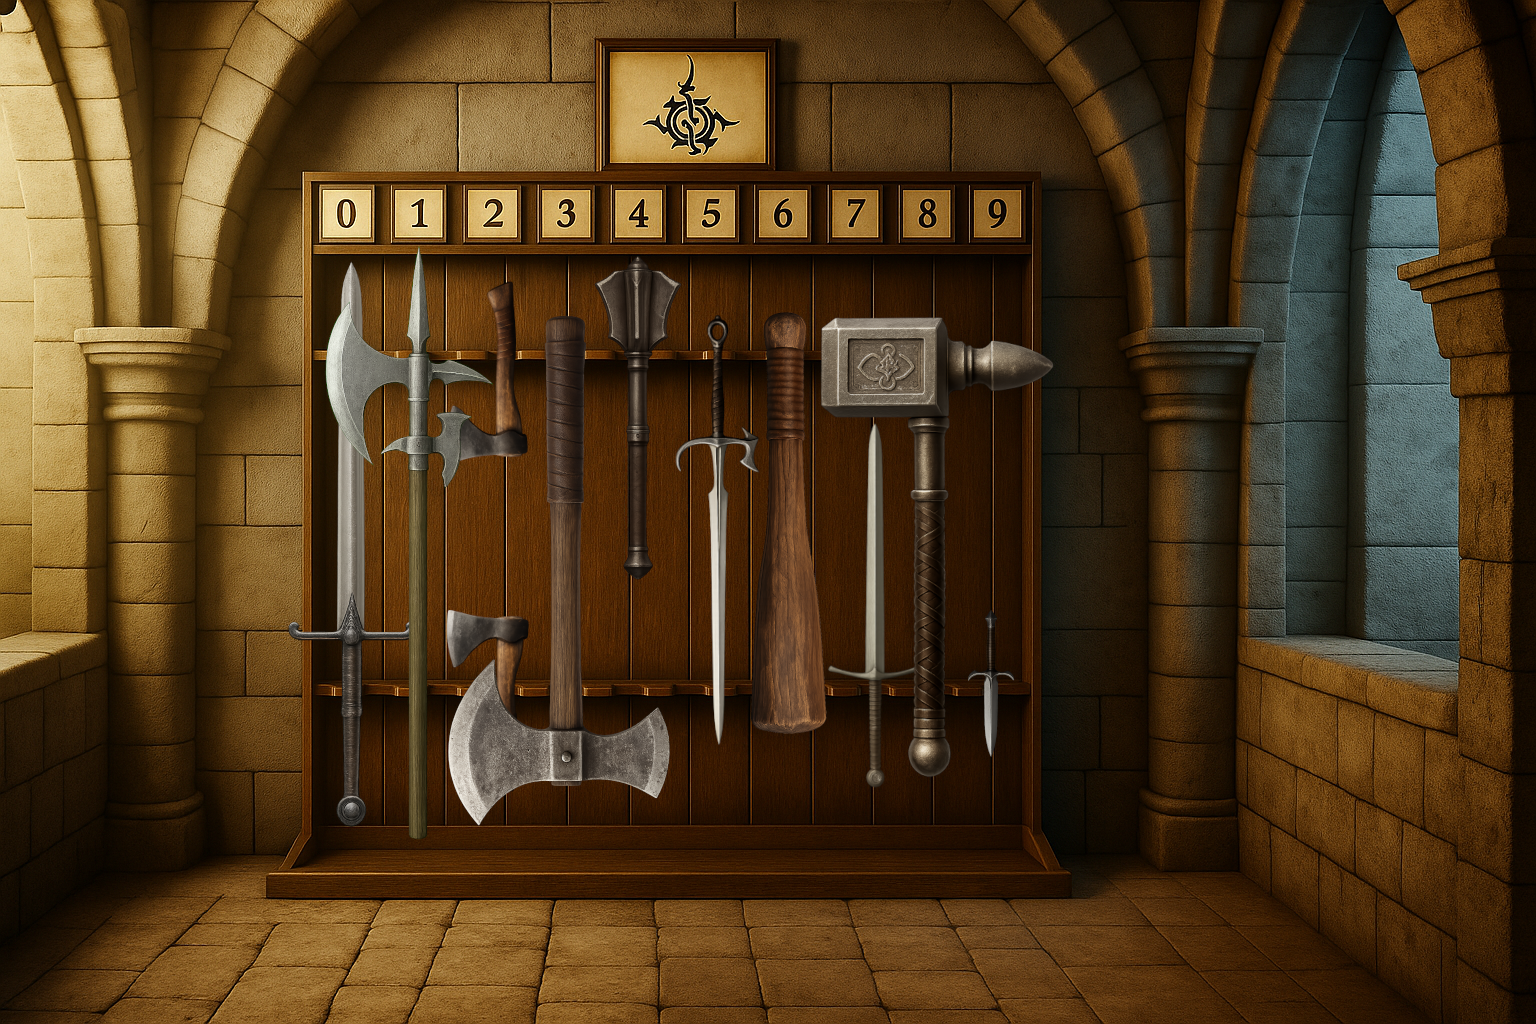
\includegraphics[width=\linewidth]{Puzzles/Weapon_Rack}

{\noindent\entryfont On this weapon rack, each number corresponds to a specific weapon: 4 is the mace, 9 is the dagger, and 7 is the longsword. To determine the proper order, players must arrange these three weapons by their damage dice - in ascending order from lowest to highest.}

\section*{Headmaster's Arcanum}\phantomsection\addcontentsline{toc}{section}{Headmaster's Arcanum}
{\entryfont The Arcanum is an impeccably maintained study, its polished marble floor reflecting the soft glow of arcane sconces. Every shelf and cupboard is completely void of books and artifacts, as though each volume was removed with deliberate care mere hours ago. There are no scuff marks or signs of disorder - only faint impressions on the dustless surfaces where tomes once rested. Drawers are closed flush, and the velvet rug lies perfectly centred before the fireplace. The sole remaining object is a leather-bound volume titled \textbf{"On the History of Master Arcanists"}, placed deliberately in the center of the mahogany desk. The lingering scent of fresh ink and parchment suggests Professor Ambric organized the space recently, then departed.}
\begingroup
	\DndSetThemeColor[PhbLightGreen]
	\begin{DndComment}{On the History of Master Arcanists}
		\textit{A book containing the history and description of the following spells:
		\begin{itemize}
			\item Jim's Magic Missile
			\item Melf's Acid Arrow
			\item Melf's Minute Meteor
			\item Leomund's Secret Chest
		\end{itemize}
		These spells can be copied into a spellbook.}
	\end{DndComment}
\endgroup
\chapter*{Wedding Ceremony}\stepcounter{chapter}\phantomsection\addcontentsline{toc}{chapter}{Wedding Ceremony}
\DndDropCapLine{W}{\entryfont ith the Grand Joust concluded and the dust of the arena settled, the realm turns its eyes toward the Wedding Ceremony. Nobles and warriors, emissaries and jesters, all gather beneath the soaring banners of the Kingdom of Fife, bearing witness to the sacred union that will shape the future of the land.}

{\entryfont The air is filled with the soft melodies of minstrels, the quiet murmur of conversation, and the distant toll of ceremonial bells. The feast is prepared, the finest ales poured, and every detail has been arranged to honour this momentous occasion. As the ceremony begins, the weight of history settles upon those in attendance - this is more than a union of two souls; it is a bond that will shape the future of the realm.}

\subsection*{Lost Bet}
{\entryfont Should a player have lost their bet with Ser Proletius their fate is now inescapable. The grandmaster, ever the showman, seizes the moment, throwing a jubilant arm around the unlucky soul and pulling them toward the center of the stage.}
\begin{DndReadAloud}
	\textit{"A debt is a debt, my friend!"} Proletius declares, his voice booming over the gathered guests. \textit{"And tonight, we shall hear your voice in all its glory!"}

	With a grand gesture, he signals the minstrels, who immediately begin playing the first triumphant notes of \textbf{The Anthem of Crail}. The crowd erupts in cheers, awaiting your performance - whether you sing with the heart of a true Knight of Crail, fumble awkwardly through forgotten lyrics, or attempt some last-ditch trickery to escape your fate.
\end{DndReadAloud}

\section*{Dwarven Keg of Chaos}\phantomsection\addcontentsline{toc}{section}{Dwarven Keg of Chaos}
{\entryfont A relic of mirth and mystery, the Dwarven Keg of Arcane Chaos is a legendary wedding tradition among the dwarves of the Mines of Methven, nestled deep within the western mountains of the Kingdom of Fife. Said to have been crafted by the Brewlords of Old, the keg is not bound by mortal hands - instead, it is infused with the raw, unpredictable essence of arcane fermentation.

The Methven dwarves believe that drinking from the keg is a blessing of fortune and folly alike - a way for fate to weave its hand into the revelry of a grand occasion. No two drinks are ever the same, and those who partake may find themselves endowed with temporary gifts, burdened by absurd curses, or simply confused as to why they now possess a perfectly baked meat pie.

It is tradition among the dwarves that the keg be brought forth at grand unions and feasts of great joy, for a wedding without chaos is a wedding doomed to boredom. Legends claim the first Grandmaster of Crail himself drank from its frothy depths and spent an entire evening levitating uncontrollably while composing a ballad about cheese wheels - a song still sung in dwarven halls to this day.}
\begin{tikzpicture}[remember picture, overlay]%
	\node[xshift=0.25cm, yshift=-0.25cm, anchor=south east] at (current page.south east) {\includegraphics[width=.5\paperwidth]{%
		images/Props/Pocket_Meat_Pie%
	}};%
\end{tikzpicture}%
\begin{DndTable}[header=Magical Effects]{cX}
	1d10	& Effect \\
	1 		& \textbf{Beard of Glory}\newline You grow a magnificent beard, regardless of gender. For the next hour you have advantage on Charisma (Persuasion) rolls.\\
	2		& \textbf{Tongue of the Brewlord}\newline For the next 5 minutes you can only speak, read and understand Dwarven. (Primordial if you already can speak and understand Dwarven)\\
	3		& \textbf{The Floor is Lava!}\newline You think that the whole floor is lava. You have to jump from object to object to move through the room. If you touch the floor in any way, you take \DndDice{1d4} Psychic damage. This effect persists for 1 minute or until you take damage.\\
	4		& \textbf{Mithral Stomach}\newline For 1 hour you are immune to poison - even alcoholic poisoning - and can eat anything.\\
	5		& \textbf{Jolly Jig}\newline A random dwarven drinking song fills your mind. You must make a DC 12 Wisdom Saving Throw or dance and sing for the next minute.\\
	6		& \textbf{Echoing Belch}\newline Your next burp is so loud that it can be heard 300 feet away. Small or tiny creatures that can hear the burp must succeed on a DC 15 Wisdom Saving Throw or are frightened for 1 minute.\\
	7		& \textbf{Dwarven Gourmet}\newline For the next 10 minutes you have developed an absolute love for the dwarven cuisine. You may demand for ale-soaked mushrooms, stone-bread, or lava-boiled snails for the duration of this effect.\\
	8		& \textbf{Mysterious Pocket Snack}\newline You find a still warm meat pie (\DndDice{2d4 + 2} Temporary Hit Points when eaten) in your pocket. How did it get there? It smells delicious.\\
	9		& \textbf{Bard's Curse}\newline For the next 5 minutes whenever you try to speak, you instead sing your words in a dramatic ballad-like fashion.\\
	10		& \textbf{Blessing of the Brewlords}\newline A faint golden glow surrounds you. For the next hour you have advantage on Charisma Checks when dealing with dwarves. Also, dwarves will offer you free drinks.
\end{DndTable}

\vfill\eject

\section*{Seer's Confection}\phantomsection\addcontentsline{toc}{section}{Seer's Confection}
{\entryfont At the heart of the wedding feast, standing upon a pedestal of ornate silver and enchanted stone, rests a cake of mysterious origin and whispered legend. Though no one can say exactly where it came from, it is known to appear only at the most significant unions in history - always present, yet never explained. Some believe it to be the work of the Cairngorm Wizards, the enigmatic spellcasters of the western reaches, while others insist it is a creation of fate itself, woven from threads of time and possibility.

The nobility refer to it in hushed tones as \textit{"The Seer's Confection"}, a name that carries both awe and caution. The legends claim that those who partake will experience visions of their destiny, glimpsing possible futures - some glorious, some tragic, some utterly incomprehensible. However, fate does not reveal itself lightly, and the cake's magic is not without risk.}
\begin{DndTable}{cX}
	1d100	& Vision/Effect \\
	1 		& You fall into a \textit{Destiny Coma}. When the player is woken up he speaks the words of \textbf{"Anstruther's Dark Prophecy"}, but cannot recollect the words or the reason why afterwards.\\
	2-20	& \textit{Destiny Coma}\\
	21-40	& \textit{You glimpse the rippling surface of a vast, mist-covered lake, just as something massive and serpentine slips beneath the water - too distant to see clearly, yet leaving behind an unnatural stillness that lingers long after the vision fades.}\\
	41-60	& \textit{In the far corner of the Braided Unicorn Tavern, half-hidden beneath a worn, dust-covered rug, you glimpse the outline of a trapdoor - its edges marked by age and secrecy. A faint draft of cold, earthy air whispers from its seams, hinting at a tunnel descending into darkness.}\\
	61-80	& \textit{You see a woven basket resting tipped over on the earth - its lid lying next to it - near the edge of what appears to be the early foundations of the city of Dundee, silent and bathed in golden morning light.}\\
	81-99	& You have a vision of three items: a Battlehammer, an Amulet, and a Dagger.\\
	100		& You speak the words of \textbf{"Anstruther's Dark Prophecy"}.
\end{DndTable}
\subsection*{The Destiny Coma}
{\entryfont For some, the sheer magnitude of the destinies they witness is too much to bear. Their minds become lost in the flood of possibility, their bodies collapsing into unconsciousness as they struggle to grasp what they have seen. This state, known as the Destiny Coma, has struck down kings, knights, and scholars alike. While most awaken quickly with aid, some never return at all, their minds forever lost in the depths of fate's tapestry.

Should one succumb to the Destiny Coma, they experience the following effect:}
\begingroup
	\DndSetThemeColor[PhbMauve]
	\begin{DndComment}{Destiny Coma}
		\textit{You are overwhelmed by the many destinies you see and fall unconscious, taking \DndDice{1d6} Psychic damage. You can only be woken up by a healing spell/potion - a Goodberry is sufficient - or you are hit after 1 minute of being unconscious, taking at least 1 bludgeoning damage.}
	\end{DndComment}
\endgroup

\vfill\eject

\section*{Floating Goblets}\phantomsection\addcontentsline{toc}{section}{Floating Goblets}
\begin{tikzpicture}[remember picture, overlay]%
	\node[xshift=0.25cm, yshift=0.25cm, anchor=north east] at (current page.north east) {\includegraphics[width=.25\paperwidth]{%
		images/Props/Hobgoblet_Shuffleboard%
	}};%
\end{tikzpicture}%
{\entryfont Tucked into a shadowed corner of the bustling\\grand plaza, a small table draws a lively crowd.\\ Laughter, cheers, and playful jeers rise above\\the din, as people gather around what appears\\to be a simple game - yet there's a spark of\\excitement, and perhaps mischief, in the air.

The "stall" is hosted by the charismatic\\Lady Belissa and the quick-tongued Sir Alrik the Swift, both commanding the crowd with practised flair and contagious energy. However, beneath their convincing appearances, these two are in fact the notorious Breeza and Arlen in masterful disguise.

Only a successful DC 30 Wisdom (Insight) Check reveals subtle clues - a familiar piece of jewelry worn by "Belissa", or a fleeting speech quirk in "Alrik's" banter - hinting at their true identities beneath the disguises. To everyone else, they remain just another pair of colourful revellers adding their own brand of excitement to the festivities.}

\subsection*{The Hobgoblet Shuffleboard}
{\entryfont A Player Character and Alrik (Sleight of Hand +2) each take turns sliding a goblet down the polished table (Dexterity Sleight of Hand Check), aiming for marked scoring zones at the far end. The goal is to accumulate the highest total score over three rounds.}

\begin{DndTable}[header=Shuffleboard Scoring]{lXX}
\textbf{Roll}	& \textbf{Location}		& \textbf{Points}		\\
less than 8		& Too Short				& 0						\\
8+				& First Zone			& 1						\\
12+				& Second Zone			& 2						\\
16+				& Third Zone			& 3						\\
NAT20			& Right on the Edge		& 3	- chance to cheat	\\
20+				& Too Long				& 0						\\
\end{DndTable}

{\entryfont \paragraph*{Cheating} The hosts still cannot move away from their cheating ways and again created a sophisticated cheating mechanism to turn the odds in their favour. The table can be tilted by Belissa to ensure a goblet either moving further - even off the table - or stopping earlier than expected.

Whenever Sir Alrik takes his turn, Lady Belissa subtly tilts the table at just the right moment, allowing her to adjust Alrik’s roll by up to $\pm 4$. Additionally, if an opponent rolls a natural 20, Belissa can discreetly interfere - shifting the balance of the table just enough to cause the goblet to veer off and fall, nullifying what would have been a perfect shot.

The player or a bystander can notice this kind of cheating with a successful DC 15 Wisdom (Perception) Check and possibly intervene.}\\\\
{\entryfont \paragraph*{Fleeing Revellers} If the players catch Belissa and Alrik cheating, they slip into the crowd and vanish, leaving behind a small pouch of valuables:
\begin{itemize}
	\item 75GP
	\item Cantrip Scroll of Minor Illusion
\end{itemize}
}

\vfill\clearpage

\section*{Encounters}\phantomsection\addcontentsline{toc}{section}{Encounters}
{\entryfont As the ceremony turns to celebration, the wedding feast offers a rare chance to speak with key figures of great importance. Conversations held tonight may reveal hidden truths, forge alliances, or stir tensions yet unseen.}

\subsection*{Prince Angus McFife}
{\entryfont On this day, Prince Angus McFife is the happiest man in the world. His love for Iona McDougall is evident in every word he speaks, every glance he steals in her direction. He radiates joy, pride, and an unwavering belief in the future, knowing that their union will bring peace and prosperity to the kingdom.

Angus is genuinely pleased to see so many people from all corners of Fife gathered for the festivities. Unlike many nobles, he is deeply interested in the lives of others, eagerly asking the party about their backgrounds, their adventures, and what brought them to this moment.}
\subsubsection*{Stance on the Highland Mysteries}
{\entryfont Angus does not dismiss the danger, knowing that people - real people - have died or gone missing, even if the stories themselves are exaggerated or wrapped in legend. What frustrates him most is his father's reluctance to act, as King Dundax \RoyalRoman{XIII} sees the tales as nothing more than superstitious nonsense.

Angus knows arguing with his father is futile, but that does not mean he does nothing. If he cannot fight the cause directly, he will fight for and support the families left behind.}
\subsection*{King Dundax \RoyalRoman{XIII}}
{\entryfont The esteemed ruler of the Kingdom of Fife, King Dundax \RoyalRoman{XIII}, welcomes conversation with a regal yet measured presence. He speaks at length about the history of the kingdom, its alliances, and the broader landscape of power across the land. His focus remains on matters of diplomacy, legacy, and the future of Fife, offering insights into the realm's political state and its standing among neighbouring territories.}
\subsubsection*{Stance on the Highland Mysteries}
{\entryfont When the topic of strange sightings in the Highlands arises he reacts with mild amusement and scepticism. Dismissing them as superstitious nonsense, he considers such tales to be nothing more than the fancies of fearful peasants or exaggerations from overzealous hunters. He expresses no real concern, seeing no reason to divert attention from more pressing political matters.}
\subsection*{Ewan MacRae of Dunkeld}
{\entryfont If a party member faced Ewan MacRae in the Grand Joust, the stalwart protector of Dunkeld greets them with genuine admiration, praising their skill and courage in battle. He remarks that it's rare to meet someone who can truly hold their own, offering an invitation to share a drink in good company.

Ewan proves to be a welcoming and honourable man, eager to speak of his beloved city of Dunkeld and the responsibility he bears in protecting its people. He takes great pride in his duty, ensuring that the city remains safe from both external threats and the dangers of the wilds beyond its borders.}
\subsubsection*{Stance on the Highland Mysteries}
{\entryfont When asked about the mysteries of the Highlands, Ewan's expression darkens for a moment as he falls into deep thought. In a quieter voice, he admits that the hunters of Dunkeld have spoken to him about strange occurrences in the mountains and forests that lie beyond the kingdom's heartlands. Their stories are too detailed, too consistent, to be dismissed as mere folklore.

Yet, Ewan is no fool - he knows that openly speaking about such matters would invite scepticism and ridicule. Instead, he keeps his concerns private, though he remains curious and watchful, eager to uncover the truth behind whatever truly lurks in the Highlands.}
\subsection*{Princess Iona McDougall}
{\entryfont \paragraph*{Bobo was rescued} If the party successfully rescued Bobo, Iona McDougall seeks them out personally, her usual composed demeanour replaced by genuine gratitude. She expresses her deep appreciation for their actions and rewards them with a \hyperref[magicalitem:HeartPureOfSteel]{\LinkFont{Heart pure of Steel}}, ensuring they know how much their deed means.}
{\entryfont \paragraph*{Bobo is still missing}
If the party failed to rescue Bobo, her tone is far more solemn. She informs them that while Angus McFife does not outwardly show his grief, she can see the weight of his sorrow beneath the surface. The loss has affected him deeply, and though he will never speak of it, his heart is heavy.}
\subsubsection*{Stance on the Highland Mysteries}
{\entryfont Iona is concerned not for the strange sightings themselves, but for the people who have vanished - hunters, adventurers, and those who set out never to return. She worries for the families left behind, the unexplained absences, and what may be lurking in the Highlands. However, as for the stories of "rabid" unicorns and other legends, she remains largely indifferent, dismissing them as embellishments on a real and more troubling reality.}
\subsection*{Grandmaster Ser Proletius}
{\entryfont A conversation with Ser Proletius is never a quiet affair. The Grandmaster of the Knights of Crail speaks with unshakable pride about his order, boasting of their glorious deeds, unwavering honour, and unmatched skill in battle. He never misses an opportunity to praise the Knights of Crail, often weaving grand tales of past victories - sometimes exaggerated, sometimes entirely true. Despite his loud and boastful nature, he is not without humour, readily laughing at a well-placed jest and responding in kind with his own repertoire of knightly jokes and tales.}
\subsubsection*{Stance on the Highland Mysteries}
{\entryfont If there is a threat to the realm, Ser Proletius swears he would hunt it down and strike it down himself, should he ever uncover the truth. However, when it comes to the tales of "rabid" unicorns and other Highland legends, he finds himself torn between scepticism and caution. While he doesn't dismiss the rumours outright, he is equally unwilling to waste time chasing after ghost stories. If a true danger exists, he believes it will reveal itself soon enough - and when it does, he will be the one to put an end to it.}
\chapter*{Unicorn Invasion of Dundee}\stepcounter{chapter}\phantomsection\addcontentsline{toc}{chapter}{Unicorn Invasion of Dundee}\label{chapter:UnicornInvasionOfDundee}
\DndDropCapLine{F}{\entryfont lea-ridden bedding, creaking floorboards, and the lingering odour of stale ale and mildew - the deplorable conditions of within the Braided Unicorn are not suited for a good-nights rest. Any character who sleeps there automatically gains one level of exhaustion.}

{\entryfont Elves, constructs, and those who secured private lodging may attempt a DC 15 Constitution saving throw to resist the effects. If an elf or construct enjoyed the comfort of a private room, they make this saving throw with advantage.}

\begin{DndReadAloud}
	Your restless slumber is shattered by a deafening explosion that rocks the tavern. The ground trembles beneath you, and dust fills the air as distant screams echo through the chaos. A blinding flash outside is followed by a crack of thunder, and you see fireballs raining down from the skies.

	Through the grimy window, you glimpse a scene of pure carnage. Blackened plumes of smoke coil into the dawn sky as undead soldiers march through the flaming streets. Among them, corrupted unicorns charge through the chaos, killing and mauling the unfortunate and defenceless townsfolk.

	Another explosion shakes the tavern, and from downstairs, the frantic voice of the barkeep cries out: \textit{"They're here! The monsters are here! We're doomed!"}
\end{DndReadAloud}

\begin{DndOptionalRule}{Hasty Departure}\label{or:HastyDeparture}%
	When the party is abruptly roused by chaos in the Braided Unicorn, they may flee in haste, leaving behind non-essential adventuring gear such as rations and backpacks. They retain only their equipped items, quest essentials, gold, and perhaps a few potions.
\end{DndOptionalRule}

\section*{The Last Stand}\phantomsection\addcontentsline{toc}{section}{The Last Stand}
{\entryfont The barkeeper frantically urges the party to help barricade the tavern's two windows and the front door against the oncoming undead horde.

Each window requires two party members working together. A window will be successfully barricaded if the players succeed twice before failing twice during this skill challenge. For example, a players can make a DC 14 Strength (Athletics) or Dexterity (Sleight of Hand) check (or use appropriate tool proficiencies such as Carpenter's Tools).

If at least one window is successfully barricaded no undead will break through it on Turn 2. If both are successfully barricaded also on Turn 4 no new undead will appear.}
\subsection*{Encounter: Fight to Survive}
{\entryfont This encounter resembles a Monster Rush:
\paragraph*{Enemies} 2 \hyperref[monster:UndeadSoldier]{\LinkFont{Undead Soldiers}} appear at the start of the encounter. On initiative count 20 of each round after the first, 2 more undeads will breach through windows. At the start of the 3rd turn additionally a \hyperref[monster:CorruptedUnicorn]{\LinkFont{Unicorn}} will breach through the barricaded door and attack the barkeep. On initiative count 20 of the 5th turn the tavern is obliterated by a fireball, killing everyone within the tavern.
\paragraph*{End of Battle} The only goal is to flee through the tunnel beyond the trap door, pointed out by the barkeeper shortly before he is mauled and beheaded by the unicorn. As soon as all players reached the trap door the battle ends and the tavern is obliterated above them.}

\section*{The Fall of Dundee}\phantomsection\addcontentsline{toc}{section}{The Fall of Dundee}
{\entryfont Moments after the party enters the tunnel, a fireball crashes into the tavern above, obliterating the structure with a deafening roar. The tunnel shakes as debris collapses behind them, sealing the exit and forcing them forward towards the unknown.}

\begin{DndReadAloud}
	Emerging from the tunnel, you step into a scene of chaos and despair. The acrid stench of smoke fills your lungs, and the sky above burns with fire and crackling lightning. Flames consume the nearby buildings, casting flickering light over the main plaza of Dundee, now a battleground. Soldiers of the kingdom and a few desperate citizens fight valiantly, but they are hopelessly outnumbered by the relentless undead soldiers and grotesque, corrupted unicorns. The screams of the dying echo all around, mixing with the roars of undead beasts and the clash of steel.
	
	At the heart of the plaza, you see a familiar figure: King Dundax \RoyalRoman{XIII}, a golden figure in the darkness. His shining armor reflects the fiery glow of the battlefield as he duels several undead soldiers. With every swing of his blade, he fells another foe, standing as a beacon of courage amidst the carnage. For a fleeting moment, hope flickers in your hearts.
	
	But then it happens!

	A corrupted unicorn, its rotting flesh gleaming wetly and its glowing, jagged horn crackling with dark energy, bursts through the melee. With terrifying speed, it lowers its head and charges. The king barely has time to turn before the horn pierces through his golden breastplate, the force lifting him off the ground.

	Time seems to freeze as King Dundax \RoyalRoman{XIII}, the proud ruler of the Kingdom of Fife, collapses to the bloodstained cobblestones. His crown falls, rolling a few feet before stopping at the hooves of the monstrous beast.

	Around you, the battle continues, but it is clear: the heart of the kingdom has just been torn away. This is not just the fall of a city - it may well be the end of Fife itself.
\end{DndReadAloud}

\subsection*{Encounter: The King is Dead}
{\entryfont The corrupted unicorn and two undead soldiers that felled King Dundax \RoyalRoman{XIII} notice the party. With bloodlust in their hollow, glowing eyes, the creatures pivot from their prior target and focus on the adventurers. The undead soldiers advance in a disciplined formation, shields raised and weapons ready, while the corrupted unicorn lets out a bone-chilling, unnatural whinny, pawing the ground as it prepares to charge. The party has no choice but to fight for their survival amidst the chaos of the main plaza.

\paragraph*{Enemies} 2 \hyperref[monster:UndeadSoldier]{\LinkFont{Undead Soldiers}}, 1 \hyperref[monster:CorruptedUnicorn]{\LinkFont{Corrupted Unicorn}} (47 HP, no Teleport)

\paragraph*{Tactics} The undead soldiers will engage in combat first, aiming to tie up melee combatants while the unicorn uses its mobility to keep the party under pressure. The unicorn may charge at a spellcaster or ranged attacker after observing the battlefield.

\paragraph*{Support} If a player is hit by the Charge Attack or is hit by any attack while at 5 HP or below, \hyperref[char:SerProletius]{\LinkFont{Ser Proletius}} and \hyperref[char:AngusMcFife]{\LinkFont{Prince Angus McFife}} appear to help the party in the battle. Ser Proletius will charge in front of the attacked player and use his Divine Allegiance feature to take the hit instead. During the fight Ser Proletius heals the party members and protects them, while Prince Angus McFife fights along with them.

\paragraph*{End of Battle} If the unicorn is below 10 HP or both Undead Soldiers are dead, the battle will end and the evil wizard Zargothrax will appear (continue reading).
}
\section*{Unholy Coronation}\phantomsection\addcontentsline{toc}{section}{The Unholy Coronation}
{\entryfont The evil wizard Zargothrax, clad in robes of dark energy, makes his entrance atop a massive undead unicorn. His arrival heralds the city's fall, as fear and despair grip the defenders. The party witnesses his terrifying entrance, setting the stage for his declaration as the dark master of Dundee.}
\begin{DndReadAloud}
	A sudden chill grips the air, and the battlefield falls eerily silent for a fleeting moment, as though the city itself is holding its breath. Then, from above, a shadow spreads across Dundee, dark and foreboding.
	
	Through the smoke and fire, a figure emerges atop a towering, undead unicorn of war. The creature's skeletal form crackles with violet energy, its empty eye sockets burning with an eerie, unholy light. It moves with an unnatural grace, its very presence pressing down upon the battlefield like an unspoken command to submit. The few remaining defenders shrink back, their weapons trembling in unsteady hands.

	The unicorn's hooves land upon the bloodied stones of the plaza, sending a ripple of necrotic energy through the ground. A silence falls, not of peace, but of resignation - of finality. Then, a voice cuts through the air, cold and commanding, laced with dark amusement and absolute authority.

	\textit{"People of Dundee! Your king is dead. Your city is mine. Kneel before me, and perhaps I will grant you the mercy of undeath."}
	
	For a moment, the battlefield stands frozen, the weight of the proclamation hanging like a curse over the ruined city. Then - Ewan MacRae, bloodied but unbroken, charges through the haze of battle, sword raised high. His face is set with unshaken determination as he rushes toward the figure atop the undead steed.
	
	\textit{"FOR DUN-"}
	
	But before he can close the distance, he jerks violently mid-stride - his body convulsing as an unseen force seizes him. His sword clatters to the ground - he collapses onto the cobblestone, lifeless. No wounds mark his body. His charge ended in an instant, his final words forever unfinished.
	
	\textit{"PATHETIC MORTAL SCUM! KILL THEM ALL! FROM THIS DAY FORWARD, I, LORD ZARGOTHRAX, RULE DUNDEE!"}
	
	With these words, the sky, once pitch-black, erupts into an inferno of searing light, as if the heavens themselves burn in response to his unholy coronation.
\end{DndReadAloud}

{\noindent\entryfont The inferno in the sky is no natural phenomenon - it is a devastating barrage of fireballs, cascading down upon Dundee like the wrath of a vengeful god. The battle is over. There is no victory to be found here.}

\section*{Flee Certain Death}\phantomsection\addcontentsline{toc}{section}{Flee Certain Death}
{\entryfont As the destruction unfolds and the undead army overruns the last defences, Ser Proletius and Prince Angus McFife waste no time in shouting above the chaos - Dundee is lost. The city and townsfolk were not ready for war. To stay is to die. With no other choice, they urge the party towards the River Tay Bridge, the only remaining escape route.}

\subsection*{Navigating the Burning Ruins}
\begin{DndReadAloud}
	The streets are collapsing, buildings are crumbling, and undead soldiers prowl the alleys. You must find a safe route to the River Tay Bridge before you are trapped inside the city.
\end{DndReadAloud}
\subsubsection*{Goal}
{\entryfont Find a secure path through the fire and destruction.}
\subsubsection*{Skill Checks}
{\entryfont Each PC makes one check as it is a team effort to navigate safely through what seems like the apocalypse.}
\paragraph*{Perception (DC 12)}
{\entryfont Spot a safer, less-collapsed route through the city.}
\paragraph*{Survival (DC 12)}
{\entryfont Predict which building is closest to collapsing and avoid dangerous areas.}
\paragraph*{Acrobatics (DC 12)}
{\entryfont Leap over burning debris or collapsed rooftops to take shortcuts.}
\paragraph*{Investigation (DC 12)}
{\entryfont Identify an escape route hidden between buildings and rubble.}
\subsubsection*{Outcome}
\paragraph*{3+ Successes}
{\entryfont The party moves swiftly, avoiding unnecessary danger.}
\paragraph*{1-2 Successes}
{\entryfont The party takes some damage from falling debris (\DndDice{1d4} bludgeoning damage).}
\paragraph*{0 Successes}
{\entryfont They are caught in a collapsing street, taking \DndDice{1d4 + 2} bludgeoning damage and gaining one level of exhaustion as they free themselves from the rubble.}

\subsection*{Pass the Undead Horde}
\begin{DndReadAloud}
	As you navigate the war-torn streets of Dundee, you see a group of undead soldiers cut down fleeing townsfolk. Beyond the carnage, the River Tay Bridge stands, but to reach it, you must find a way past these relentless killers... or cut through them.
\end{DndReadAloud}
\subsubsection*{Goal}
{\entryfont Sneak past the undead horde or engage in battle, fighting your way through them and towards your escape.}
\subsubsection*{Skill Checks}
{\entryfont Each PC makes one check aiding to find a way and sneaking past the undead soldiers.}
\paragraph*{Stealth (DC 15)}
{\entryfont Weave through burning and collapsed buildings to avoid detection.}
\paragraph*{Athletics (DC 15)}
{\entryfont Smash through weakened structures to create a new escape route.}
\paragraph*{Intimidation (DC 15)}
{\entryfont Shout commands to confuse and frighten the undead.}
\paragraph*{Deception (DC 15)}
{\entryfont Trick the undead into hesitating searching for you.}
\paragraph*{Sleight of Hand (DC 15)}
{\entryfont Quickly unlock a barricaded side gate leading toward the bridge.}
\subsubsection*{Outcome}
\paragraph*{5 Successes}
{\entryfont The party finds and saves a little child hiding in the rubble (+1 Heroic Inspiration for each PC). They successfully sneak past the relentless killers.}
\paragraph*{3-4 Successes}
{\entryfont The party stealthily bypasses the enemies without combat.}
\paragraph*{0-2 Successes}
{\entryfont The undead detect the players, and the party must fight anyway (reinforcements will arrive 1 turn earlier).}
\subsubsection*{Combat}
{\entryfont If the party decides to engage in combat or are detected by the enemies they are attacked by 5 \hyperref[monster:UndeadSoldier]{\LinkFont{Undead Soldiers}} (20 HP). Angus McFife and Ser Proletius can join the battle. On Initiative Count 20 on Turn 5 reinforcements (2 \hyperref[monster:UndeadSoldier]{\LinkFont{Undead Soldiers}} and 1 \hyperref[monster:CorruptedUnicorn]{\LinkFont{Unicorn}}) will arrive - Turn 4 if the party failed to sneak past the horde.}

\subsection*{The Final Sprint over the Bridge}
\begin{DndReadAloud}
	As you near the River Tay Bridge, fireballs hammer the ancient stonework, sending tremors through the ground as chunks of masonry crumble into the raging waters below. The entire structure groans under the assault, shaking violently beneath your feet.

	From ahead, Ser Proletius and Prince Angus McFife turn back, their eyes wide with urgency.

	\textit{"MOVE NOW! RUN!"}

	A deafening crack splits the air as another fireball slams into the bridge. The supports buckle. The path behind you is collapsing.

	There is not much time to make it across...
\end{DndReadAloud}
\subsubsection*{Goal}
{\entryfont Sprint across the collapsing River Tay Bridge to reach the far side before it crumbles into the waters below. Safety is uncertain, but staying behind means certain death.}
\subsubsection*{Skill Checks}
{\entryfont This is a frantic individual challenge - each PC must rely on their own speed and reflexes to survive.
\begin{itemize}
	\renewcommand\labelitemi{\textbf{\textbullet}}
	\item \textbf{Athletics (DC 13):} For those with trained endurance, sprinting full speed across the unstable bridge while dodging fireballs (Athletics Skill Proficiency required).
	\item \textbf{Acrobatics (DC 13):} For the agile, weaving through debris and leaping across collapsing sections of stone (Acrobatics Skill Proficiency required).
	\item \textbf{Dexterity Saving Throw (DC 16):} For those untrained in either skill, relying purely on instinct to react fast enough to avoid falling rubble and crumbling pathways.
\end{itemize}}
\vfill\eject
\subsubsection*{Outcome}
{\entryfont If a character fails their check, the Degree-of-Failure (DoF) - the difference between their roll and the DC - will dictate the consequences.}
\paragraph*{Success}
{\entryfont The Player crosses the bridge exhausted but unscathed.}
\paragraph*{Failure (DoF max 5)}
{\entryfont The Player takes \DndDice{1d6} fire damage, but makes it across - if not dropped to 0 hit points.}
\paragraph*{Failure (DoF > 5)}
{\entryfont The Player falls as the bridge crumbles beneath their feet. They must make a DC 15 Strength or Dexterity Saving Throw or fall 80 feet into the river Tay - most likely killing them instantly.}

\section*{A Horrendous View}\phantomsection\addcontentsline{toc}{section}{A Horrendous View}

{\entryfont The party finds themselves on the banks of the River Tay, breathless and shaken. Behind them, the bridge has collapsed, sealing their escape and leaving behind the burning ruins of Dundee. Across the river, where once stood a proud and thriving city, now only devastation remains. Smoke and fire rise into the sky, casting an eerie glow over the shattered buildings - a grim testament to the apocalyptic destruction that unfolded.}

\begin{DndReadAloud}
	As you stand on the muddy banks of the River Tay, the weight of what just transpired settles heavily upon you. Across the water, Dundee is no more. The once-great city, its spires and halls that once shone in the golden light, is now a smoldering ruin. Smoke curls into the sky like grasping fingers, and fires rage unchecked, their glow reflected in the darkened waters of the river. The echoes of distant screams and the collapsing of buildings still carry across the wind, a final whisper of the city's last breath.

	Beside you, Ser Proletius and Prince Angus McFife stand motionless, their eyes fixed on the ruins before them. Proletius, his armour still scarred from battle, grips his sword so tightly his knuckles turn white, his usually unshakable demeanour fractured by the horror of what he has just witnessed.

	Angus McFife stares in disbelief, his face pale, his lips parted as if to speak - but no words come. His city, his people, his home... all lost. His breath quickens as his eyes scan around the few survivors, searching, hoping for a glimpse of something - of someone. But there is no sign of Iona McDougall.

	His shoulders tense, his hands balling into fists. A new fire ignites in his eyes - not the flickering glow of sorrow, but the burning heat of vengeance. He grits his teeth, his voice shaking but firm as he finally speaks:

	\textit{"I will make Zargothrax die!"}

	The wind howls across the river, carrying with it the embers of a fallen kingdom. The city of Dundee is lost, but the fire of revenge has just been lit.
\end{DndReadAloud}

{\centering\entryfont The battle is over - the city of Dundee has fallen.\\But the war has only just begun.\\}

\begin{tikzpicture}[remember picture, overlay]%
	\node[yshift=-1cm, anchor=south] at (current page.south) {\includegraphics[width=\paperwidth]{%
		images/Landscape/Fallen_City_of_Dundee%
	}};%
\end{tikzpicture}%

{\centering\contourlength{0.05em}\Large\contour{black}{\textcolor{titlegold}{\textbf{\textsc{Level-Up}}}}\\}